\begin{figure*}[!t]
  \centering
  \subfloat[The execution time of the forward computation] {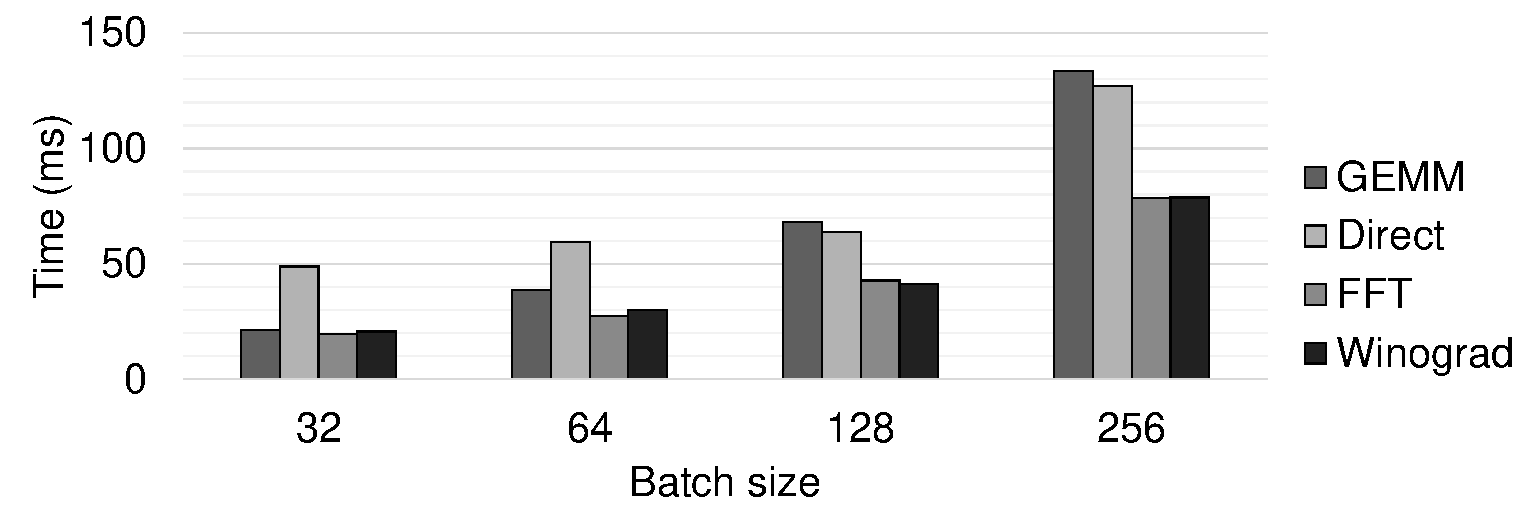
\includegraphics[width=.45\linewidth]{./figures/gpu_time_fwd}
  \label{fig_gpu_time_fwd}}
  \subfloat[The execution time of the backward computation] {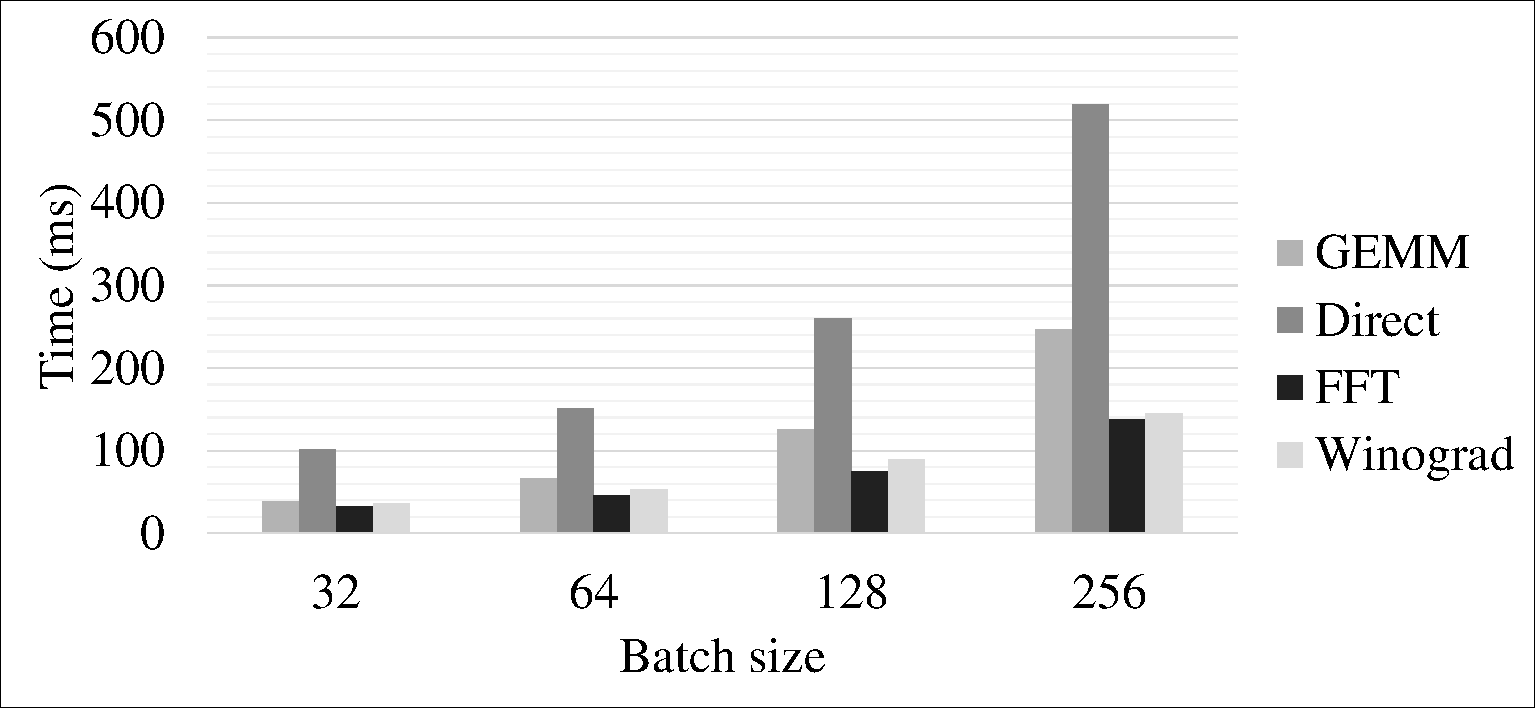
\includegraphics[width=.45\linewidth]{./figures/gpu_time_bwd}
  \label{fig_gpu_time_bwd}}
  \hfil
  \subfloat[The execution time of the forward computation from \textsf{conv3} to \textsf{conv5}] {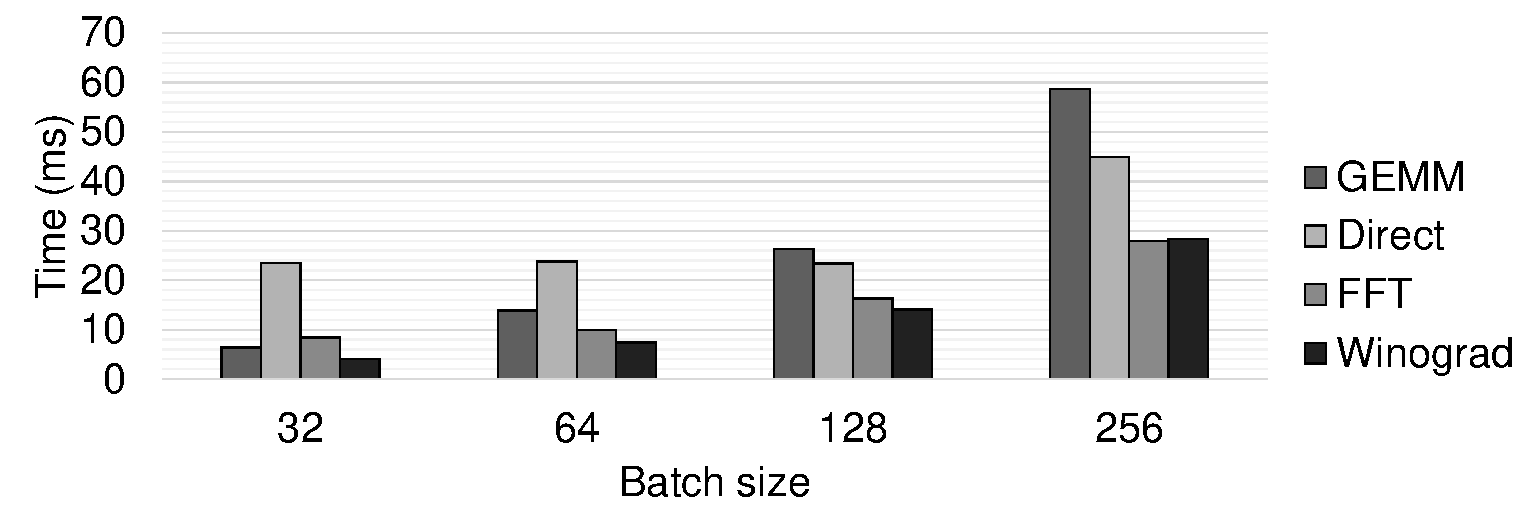
\includegraphics[width=.45\linewidth]{./figures/gpu_time_conv345}
  \label{fig_gpu_time_conv345}}
  \subfloat[Peak GPU memory usage] {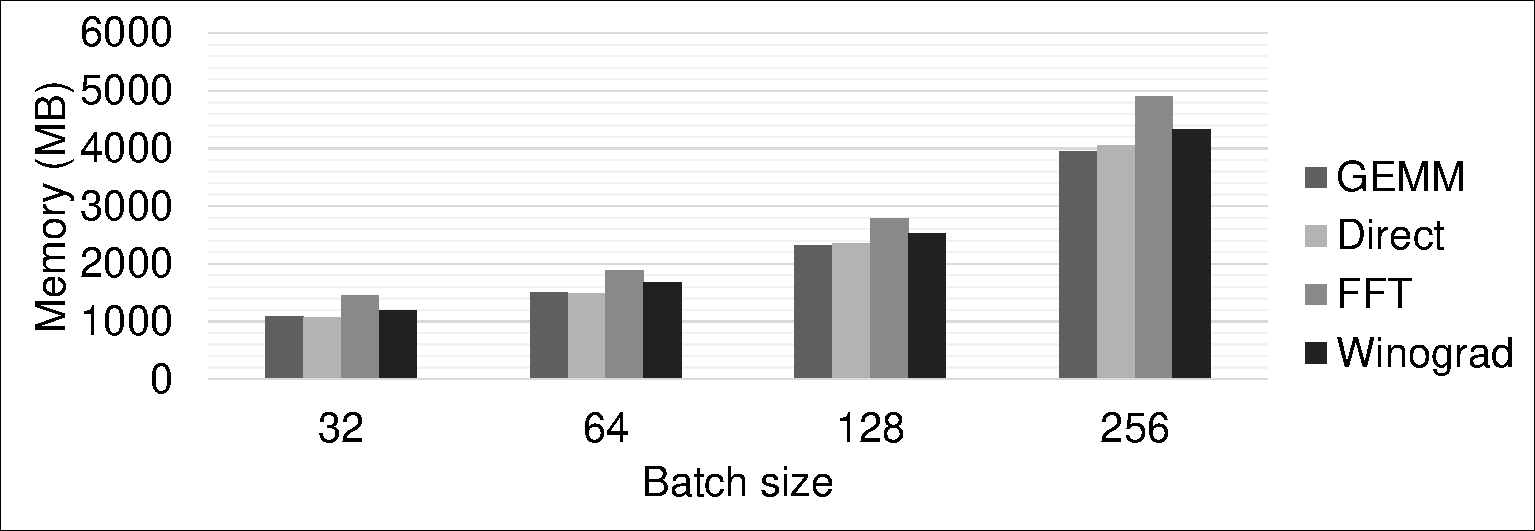
\includegraphics[width=.45\linewidth]{./figures/gpu_mem_kernels}
  \label{fig_gpu_mem}}
  \caption{Execution time and memory usage between different convolution algorithms.}
  \label{fig_conv_time}
\end{figure*}%

\section{Characterization of Convolution Algorithms}
\label{convolution-algorithms}
In this section, we compare the performance of different convolution algorithms on a single GPU. These algorithms were introduced in Section~\ref{sec:algorithms}.
We used Cuda-convnet for \textsf{Direct}, and cuDNN for \textsf{GEMM}, \textsf{FFT}, and \textsf{Winograd}.

\subsection{Execution Time of Convolution Algorithms}
Figure~\ref{fig_conv_time} shows execution time comparisons between different convolution algorithms (\textsf{GEMM}, \textsf{Direct}, \textsf{FFT}, and \textsf{Winograd}) on a single GPU. We vary the batch size from 32 to 256. Since the convolution layers take most of the execution time in a CNN, using an efficient convolution algorithm is an important design decision. All comparisons are done with the AlexNet model built by Torch7 because it is the only framework that officially supports the newest versions of cuDNN and cuda-convnet3. Randomly generated images are used for the input to remove the effect of I/O latency. The forward and backward computation times are measured and averaged for 100 iterations (\textit{i.e.}, batches). 

\textsf{Winograd} and \textsf{FFT} perform better than \textsf{Direct} or \textsf{GEMM} most of the time as shown in Figure~\ref{fig_gpu_time_fwd} and Figure~\ref{fig_gpu_time_bwd}. Since many recent CNN models use $3 \times 3$ kernel for convolution layers\cite{vgg}, the forward computation times of \textsf{conv3},  \textsf{conv4} and \textsf{conv5} are separately measured in Figure~\ref{fig_gpu_time_conv345}.

The total training time (the forward computation time + the backward computation time) of \textsf{FFT} is the best for all batch sizes. However, for $3 \times 3$ convolution kernels with a small batch size, \textsf{Winograd} performs better than \textsf{FFT} while \textsf{FFT} scales better with a large batch size. In addition, \textsf{Direct} (\textit{i.e.}, Cuda-convnet) scales poorly when the batch size is smaller than 128 while \textsf{GEMM} scales almost linearly.

Figure~\ref{fig_gpu_mem} shows peak GPU memory usage for each convolution algorithms. \textsf{FFT} occupies the most GPU memory, using about 20\% more memory than \textsf{GEMM}. 

\begin{figure}[htbp]
  \centering
  \subfloat[The execution time of the forward computation] {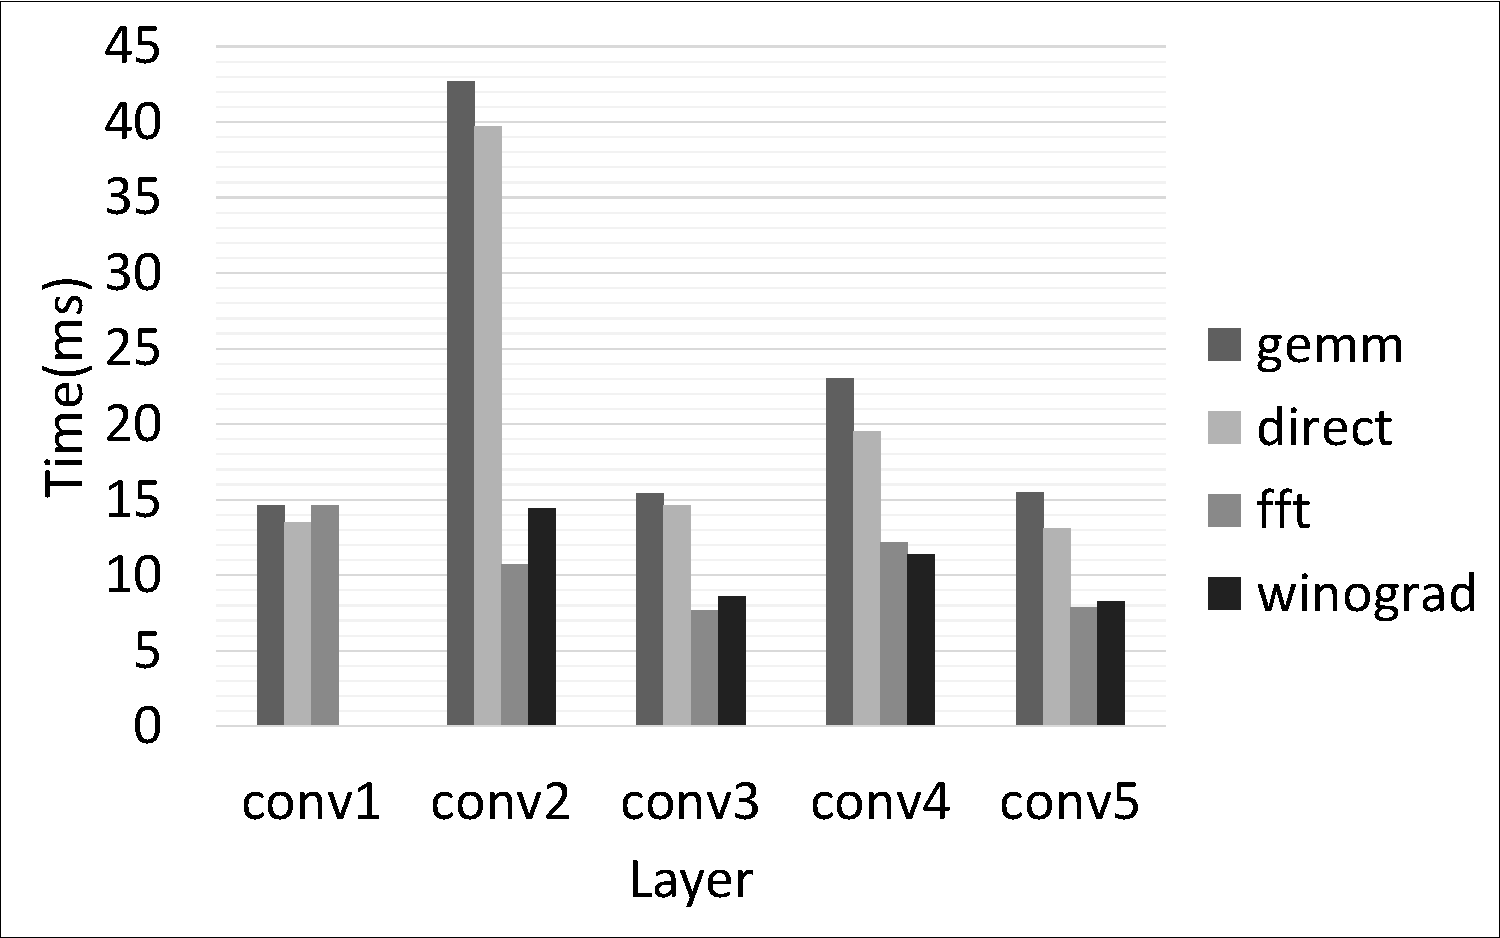
\includegraphics[width=.9\linewidth]{./figures/layerwise_fwd}
  \label{fig_layerwise_fwd}}

  \subfloat[The execution time of the backward computation] {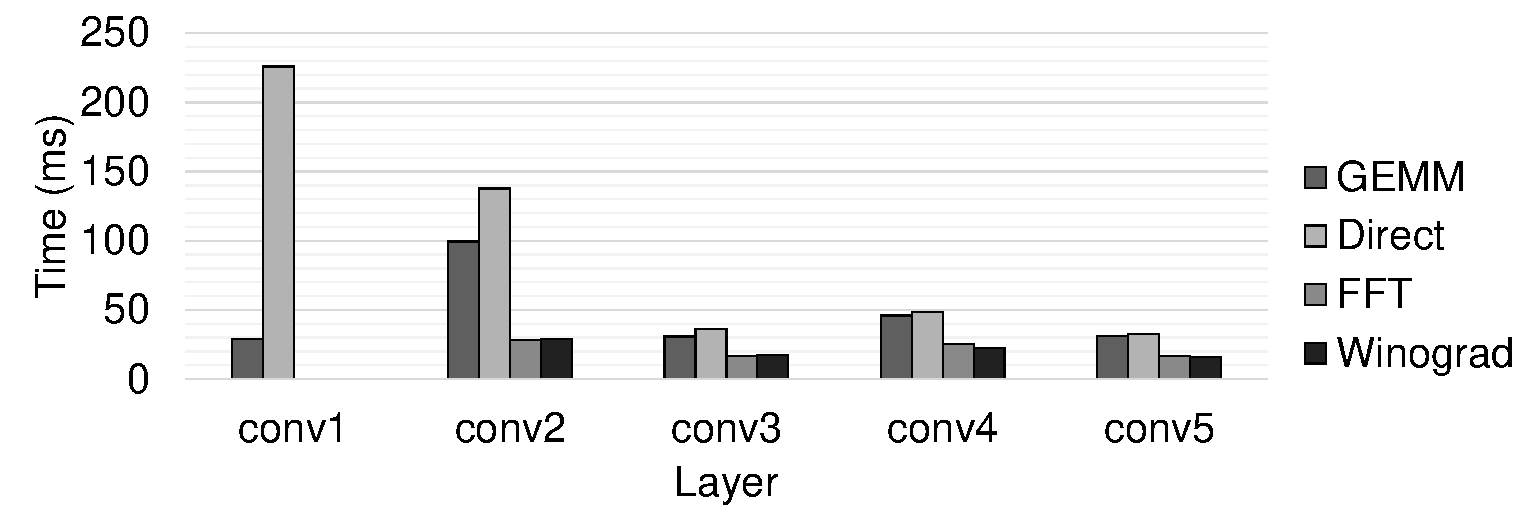
\includegraphics[width=.9\linewidth]{./figures/layerwise_bd}
  \label{fig_layerwise_bd}}

  \subfloat[FP operation count in the forward computation] {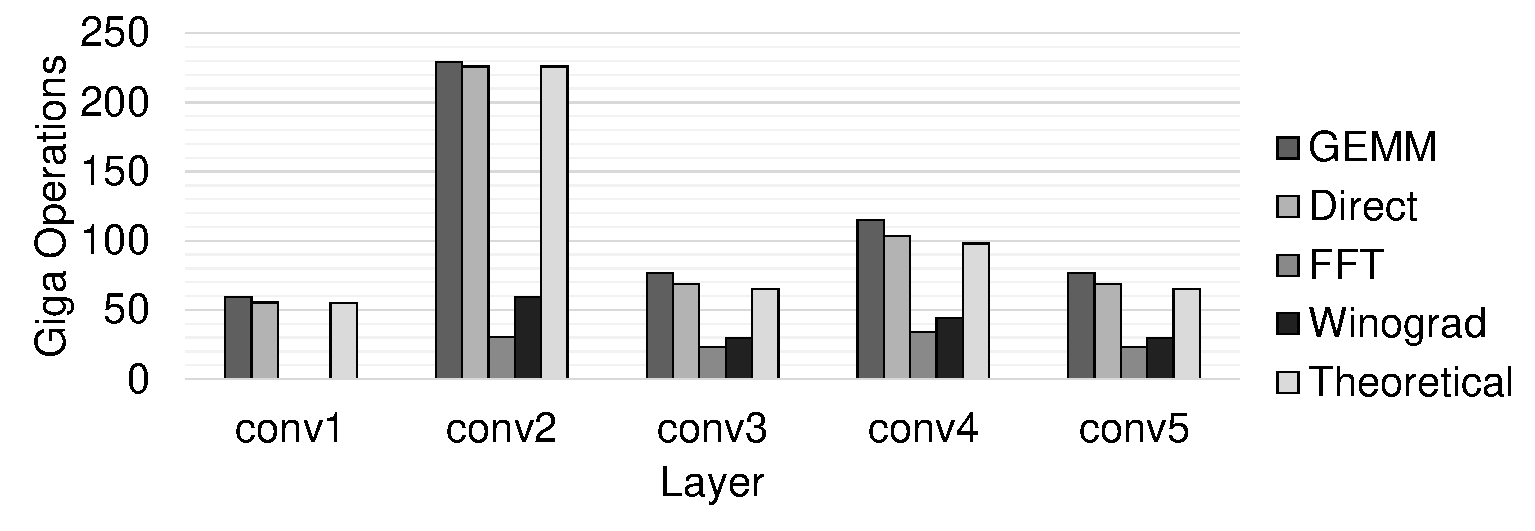
\includegraphics[width=.9\linewidth]{./figures/layerwise_flop_count}
  \label{fig_layerwise_flop_count}}

  %\subfloat[FP-operations-to-memory-accesses ratio of the backward filter convolution] {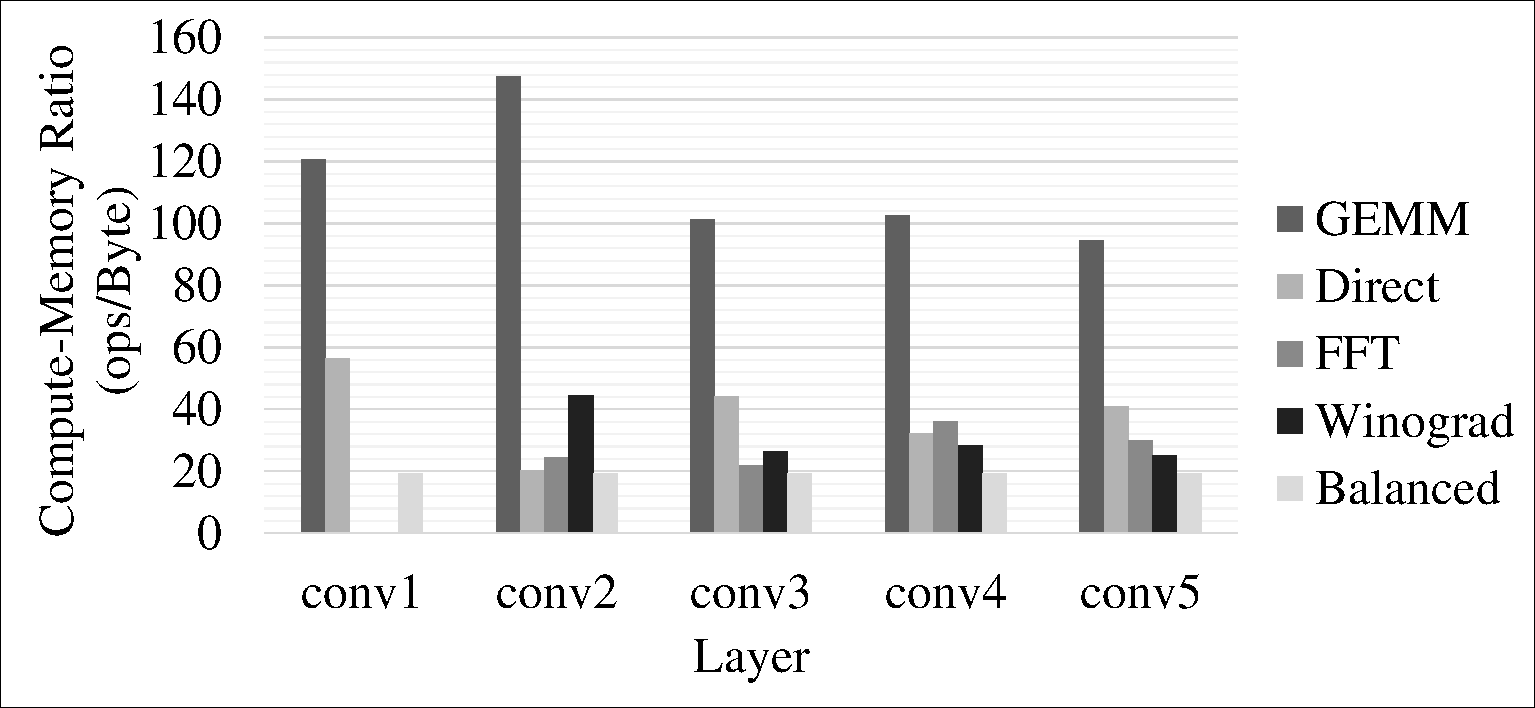
\includegraphics[width=.9\linewidth]{./figures/layerwise_mem_compute}
  %\label{fig_layerwise_mem_compute}}%compute-memory ratio chart added

  \caption{Layerwise analysis of different convolution algorithms.}
  \label{fig_layerwise}
\end{figure}

\begin{figure*}[htbp]
  \centering
  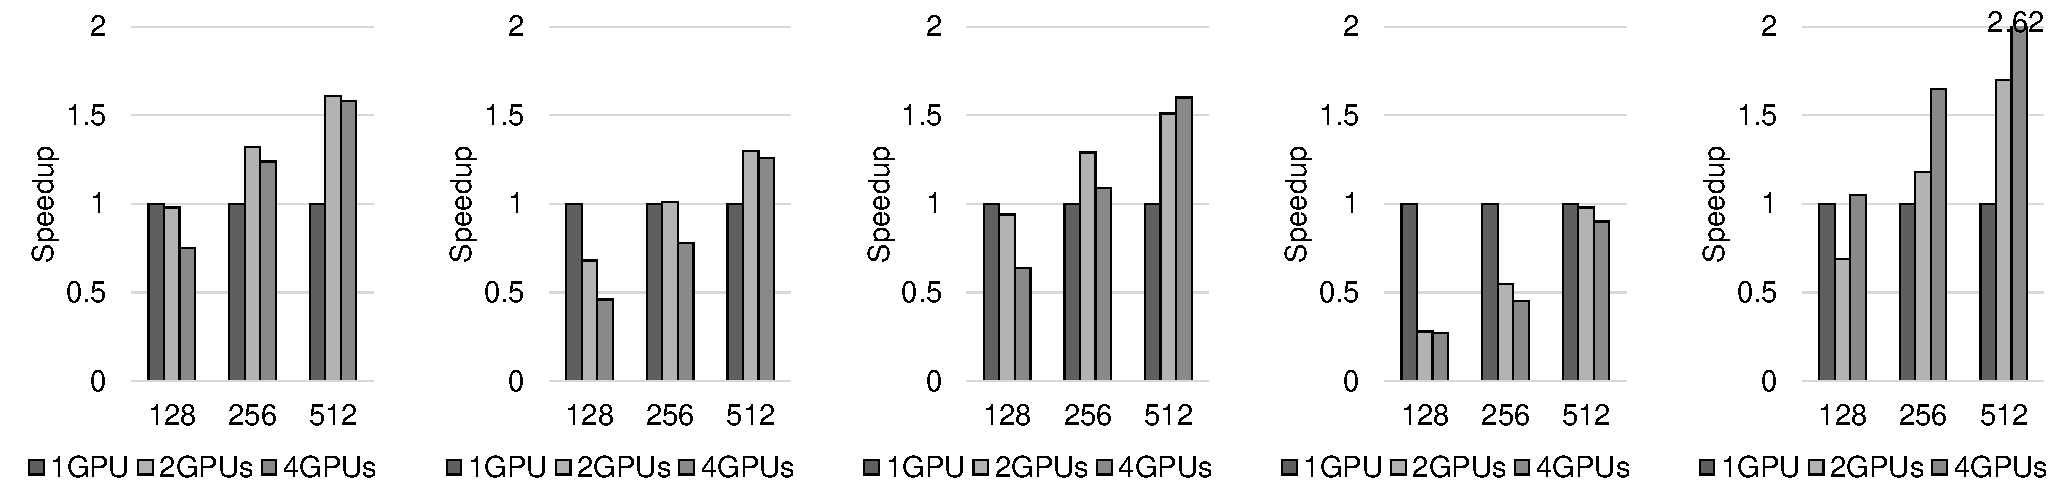
\includegraphics[width=.9\linewidth]{./figures/MG}
  \subfloat[Caffe]{\makebox[.19\linewidth][]{}}
  \subfloat[Torch]{\makebox[.19\linewidth][]{}}
  \subfloat[TensorFlow]{\makebox[.18\linewidth][]{}}
  \subfloat[CNTK]{\makebox[.18\linewidth][]{}}
  \subfloat[CNTK 1bit-SGD]{\makebox[.18\linewidth][]{}}
\caption{Speedup (over a single GPU) of multi-GPU training of the AlexNet models.}
\label{fig_mg}
\end{figure*}

\subsection{Layer-wise Analysis}

Figure~\ref{fig_layerwise} shows layer-wise analysis of different convolution algorithms on a single GPU. The batch size is set to 256, and the NVIDIA nvprof profiler is used to gather statistics. \textsf{FFT} and \textsf{Winograd} cannot be applied to the \textsf{conv1} since it has a stride size of 4. As shown in Figure~\ref{fig_layerwise_bd}, the main performance limiter of \textsf{Direct} (\textit{i.e.},cuda-convnet3) is the backward computation in \textsf{conv1} layer. The reason of the slowdown is low parallelism in \textsf{Direct} that implement \textsf{conv1} layer. While NVIDIA Titan X has 3072 CUDA cores, the number of CUDA threads in the implementation is only 1024. This makes \textsf{Direct} slower than other algorithms in \textsf{conv1}. 

%{\bf Backward and forward convolutions}. The backpropagation in a convolution layer requires two convolutions: backward data convolution (\textsf{BDC}) and backward filter convolution (\textsf{BFC}). \textsf{BDC} generates gradient input to the previous layer while \textsf{BFC} updates the parameters of the current layer. Since backpropagation requires two convolutions, the backward computation time should be double the forward computation time. Moreover, the backward computation is more memory intensive than the forward computation because \textsf{BFC} needs to update the network parameters.

{\bf Floating-point operation counts}. Figure~\ref{fig_layerwise_flop_count} compares floating-point (FP) operation counts of different algorithms in the forward computation. The count in the backward computation is double the count in forward computation. \Comment{$<$=== Check it! ===} The numbers are measured with the NVIDIA nvprof profiler. The result tells us that \textsf{FFT} is usually the fastest because of much less FP operation count (\textit{i.e.}, much less algorithm complexity). Especially, \textsf{FFT} is much faster than others in \textsf{conv2} with $5 \times 5$ convolution filter because the complexity of \textsf{FFT} does not depend on the filter size. \textsf{Winograd} also reduces FP operation count by more than a half. Thus, its performance is comparable to \textsf{FFT} in the layers with $3 \times 3$ convolution filters (\textsf{conv3}, \textsf{conv4}, and \textsf{conv5}).

%{\bf FP operations to memory accesses ratio}. The theoretical maximum FP throughput of NVIDIA Titan X is 6 TFLOPS (floating-point operations per second), and its maximum memory bandwidth is 336 GB/s. Thus, a well-balanced FP-operations-to-memory-accesses ratio is 18.3 FLOPs/B. Fig~\ref{fig_layerwise_mem_compute} shows these ratios of \textsf{BFC} algorithms and the well-balanced ratio (\textsf{Balanced}). Since the forward computation and \textsf{BDC} are less memory intensive than \textsf{BFC}, the result indicates that \textsf{FFT} and \textsf{Winograd} are compute intensive on a GPU rather than memory intensive. Thus, reduced computation complexity of \textsf{FFT} and \textsf{Winograd} result in faster convolution computation.

Overall, \textsf{FFT} and \textsf{Winograd} outperform \textsf{GEMM} or \textsf{Direct} because of their reduced algorithm complexity. \textsf{FFT} scales better with a large batch and filter size while \textsf{Winograd} scales better with a small batch and filter size. Carefully choosing a convolution algorithm can make the CNN more than 4X faster in convolution layers. 
